\documentclass[../main.tex]{subfiles}
 
\begin{document}
	\section{Physical Quantities, Units and Measurement}
		\begin{preamb}
		Measurement is a tool that we use in physics a lot. It is difficult to get fully accurate measurements due to how well we can create instruments, control random errors, and other factors. Nonetheless we try to minimise these errors by practising proper measurement techniques. We use measurements to determine physical quantities, and these quantities are communicated with units.
		\end{preamb}
			
		\subsection{Physical Quantities}
		\pdef{Physical Quantity}{A physical quantity is a quantity consisting of a \textbf{numerical magnitude} and a \textbf{unit}.}
		
		The numerical magnitude tells us the size of the quantity, and the unit tells us what the quantity is expressed in.
		
		Physical quantities can be either a \textbf{basic quantity}):
		\begin{center}
			\begin{tabular}{cccc}
				\hline \hline
				\multicolumn{2}{c}{Physical Quantity} & \multicolumn{2}{c}{SI Unit} \\
				\hline 
				mass & $m$ & kilogram & kg \\
				time & $t$ & second & s \\
				temperature & $T$ & kelvin & K \\
				length & $l$ & metre & m \\
				current & $I$ & ampere & A \\
				amount & $n$ & mole & mol \\
				\hline \hline
			\end{tabular}
		\end{center}
		or a \textbf{derived quantity}, which are derived from basic quantities. 
		
			\subsubsection{Dimensional Analysis}
			This is not explicitly taught in syllabus, but it is a very important tool to help you if you are stuck in a problem. 
			
			The main idea is to treat units like \textbf{algebraic terms}, and manipulate them accordingly to get the right derived unit for the quantity. Usually, a single unit is written in square brackets [ ] to avoid confusion with units with multiple letters (\textit{e.g.} [\si{\mole}] and [\si{\meter}]).
			
		\subsection{Prefixes, Standard Form, and Order of Magnitude}
		If a number is too large or too small, it will get very annoying to write a lot of digits. That is what prefixes and standard form aim to solve. The former will be written with the unit, while the latter will be written with the numerical magnitude.
		
		A number is expressed in standard form as
		\[ 
			\underbrace{A}_{\text{base}} \times \underbrace{10^N}_{\text{factor}} 
		\]
		where \(1 \leqslant A < 10\) and \(N \in \mathbb{Z}\).
		
		A unit can be rewritten with any of these prefixes preceding its symbol:
		\begin{center}
		\begin{tabular}{cccc}
			\hline \hline
			Prefix & Symbol & Factor & Order of Magnitude \\  
			\hline
			tera & \si{\tera} & \(10^{12}\) & 12 \\  
			giga & \si{\giga} & \(10^9\) & 9 \\  
			mega & \si{\mega} & \(10^6\) & 6 \\  
			kilo & \si{\kilo} & \(10^3\) & 3 \\  
			deci & \si{\deci} & \(10^{-1}\) & \(-1\) \\  
			centi & \si{\centi} & \(10^{-2}\) & \(-2\) \\  
			milli & \si{\milli} & \(10^{-3}\) & \(-3\) \\  
			micro & \si{\micro} & \(10^{-6}\) & \(-6\) \\  
			nano & \si{\nano} & \(10^{-9}\) & \(-9\) \\  
			pico & \si{\pico} & \(10^{-12}\) & \(-12\) \\ 
			\hline \hline
		\end{tabular} 
		\end{center}
	
		\subsection{Scalars and Vectors}
		
		\pdef{Scalar Quantity}{A scalar quantity has a magnitude, unit, but \textbf{no} direction.}
		\pdef{Vector Quantity}{A vector quantity has a magnitude, unit, and direction.}
		
		\subsection{Vector Addition}
		Vectors can be added by using the trigonometric method or the graphical method.
		\peqn{Magnitude of Vectors}{
		The magnitude of a vector \(\vec{\mathbf{v}}\) with components \(\vec{v_x}\) and \(\vec{v_y}\) is given by}{\left|\vec{v}\right| = \sqrt{\left|\vec{v_x}\right|^2 + \left|\vec{v_y}\right|^2}}
	
		\begin{center}
			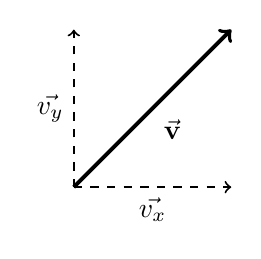
\begin{tikzpicture}
				\draw [line width=0.5mm, ->] (0,0) -- (2,2) node[anchor=north west, pos=0.5]{\(\vec{\mathbf{v}}\)};
				\draw [line width=0.25mm, dashed, ->] (0,0) -- (2,0) node[anchor=north, pos=0.5] {\(\vec{v_x}\)};
				\draw [line width=0.25mm, dashed, ->] (0,0) -- (0,2) node[anchor=east, pos=0.5] {\(\vec{v_y}\)};
			\end{tikzpicture}
		\end{center}
		\begin{center}
			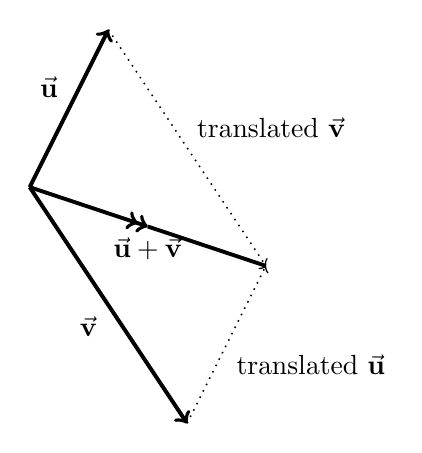
\begin{tikzpicture}
				\draw [line width=0.5mm, ->] (0,0) -- (1,2) node[anchor=south east, pos=0.5] {\(\vec{\mathbf{u}}\)};
				\draw [line width=0.2mm, dotted, ->] (2,-3) -- (3,-1) node[anchor=north west, pos=0.5] {translated \(\vec{\mathbf{u}}\)};
				\draw [line width=0.5mm, ->] (0,0) -- (2,-3) node[anchor=north east, pos=0.5] {\(\vec{\mathbf{v}}\)};
				\draw [line width=0.2mm, dotted, ->] (1,2) -- (3,-1) node[anchor=south west, pos=0.5] {translated \(\vec{\mathbf{v}}\)};
				\draw [line width=0.5mm, ->>] (0,0) -- (1.5,-0.5) node[anchor=north] {\(\vec{\mathbf{u}} + \vec{\mathbf{v}}\)};
				\draw [line width=0.5mm] (1.5,-0.5) -- (3,-1);
			\end{tikzpicture}
		\end{center}
		
		\subsection{Measurement}
		\subsubsection{Precision and Accuracy}
		
		\textbf{Precision} is how well a set of readings of the same physical quantity agree with each other.
		
		\textbf{Accuracy} is how close the set of readings are to the true value.
		
		\subsubsection{Measurement of Lengths}
		Parallax error should be avoided when measuring lengths. In the case of a measuring tape or a metre rule, the object needs to be \textbf{in contact} with the measuring instrument.
		
		\subsubsection*{Vernier Callipers}
		Accuracy: \(\pm \SI{0.01}{\centi\meter}\)
		\begin{enumerate}
			\item Check for zero error. This error is \(\Delta x\).
			\item Place the object to be measured at the appropriate measurement site (internal jaws, external jaws, or tail).
			\item Slide the vernier scale so that the jaws or tail measure the entirety of the object.
			\item On the main scale (with \SI{0.1}{\centi\meter} subdivisions), take the reading that is on or left of the `0' mark of the vernier scale, \(x_\mathrm{main}\).
			\item On the vernier scale (with \SI{0.01}{\centi\meter} subdivisions), read the mark that coincides with a mark on the main scale,\(x_\mathrm{vernier}\).
			\item The measurement is the sum of the reading on the main scale and vernier scale, and then subtracting the zero error, \(x-\Delta x\) .
		\end{enumerate}
	
		\subsubsection*{Micrometer Screw Gauge}
		Accuracy: \(\pm \SI{0.001}{\centi\meter}\)
		\begin{enumerate}
			\item Check for zero error. This error is \(\Delta x\).
			\item Place the object in between the anvil and the spindle.
			\item Close the jaws on the micrometer screw gauge until the object is in contact. Turn  the ratchet until a `click' sound is heard.
			\item On the datum line (with \SI{0.5}{\milli\meter} subdivisions), take the reading that is on the left of the circular scale, \(x_\mathrm{datum}\).
			\item On the circular scale (with \SI{0.01}{\milli\meter} subdivisions), take the reading that coincides with the datum line, \(x_\mathrm{circular}\).
			\item The measurement is the sum of the reading on the datum line and circular scale, and then subtracting the zero error, \(x-\Delta x\) .
		\end{enumerate}
	
		\subsubsection{Simple Pendulum}
		A simple pendulum is one on the premises that the string is massless, and the bob is a point mass.
		\peqn{Period of Simple Pendulum}{Using the approximation \(\cos \theta \approx 1 - \frac{\theta^2}{2}\), for a reasonably small \(\theta\) (angle of release),}{T = 2\pi \sqrt{\frac{L}{g}}}
		
\end{document}